% Define document class
\documentclass[twocolumn]{aastex631}
\usepackage{showyourwork}


\usepackage{natbib}
\usepackage[utf8]{inputenc}
\usepackage{amsmath}
\usepackage{amsmath,units}
\usepackage{amsmath,bm}
\usepackage{booktabs}
\usepackage{makecell}
\usepackage{xcolor}
\usepackage{graphicx}
\usepackage{acronym}
\usepackage{xspace}
\usepackage{enumitem}
\usepackage{calc}
\usepackage[caption=false]{subfig}
\usepackage{import}
\usepackage{mathtools}
\usepackage{showyourwork}
\usepackage{tikz}
\usepackage{float}
\usepackage{algorithm}
% \usepackage{algorithmic}
\usepackage{algpseudocode}

%%%%%%%%%%%%%%%%%%%%%%% COMMENTS

\definecolor{orange-red}{rgb}{1.0, 0.27, 0.0}
\newcommand{\jeff}[1]{\textbf{\textcolor{orange-red}{#1}}}
\newcommand{\ilya}[1]{\textbf{\textcolor{magenta}{#1}}}
\newcommand{\avi}[1]{\textbf{\textcolor{cyan}{#1}}}
\newcommand{\chayan}[1]{\textbf{\textcolor{green}{#1}}}
\newcommand{\resp}[1]{#1}


%%%%%%%%%%%%%%%  ACRONYMS
\acrodef{ANN}{artificial neural network}
\acrodef{DCO}{double compact object}
\acrodef{MCMC}{Markov Chain Monte Carlo}
\acrodef{MSSFR}{metallicity-specific star formation rate}
\acrodef{LVK}{LIGO--VIRGO--KAGRA}
\acrodef{GP}{gaussian process}



%%%%%%%%%%%%%%% CODE + PROJECTS
\newcommand{\project}[1]{\textsf{#1}}
\newcommand{\code}[1]{{\sc{#1}}\xspace}

\newcommand{\python}{\project{Python}}
\newcommand{\jupyter}{\project{Jupyter}}
\newcommand{\exoplanet}{\project{exoplanet}}
\newcommand{\lightkurve}{\project{lightkurve}}
\newcommand{\starry}{\project{starry}}
\newcommand{\pymc}{\project{PyMC3}}
\newcommand{\pymcextra}{\project{pymc3-ext}}
\newcommand{\celerite}{\project{celerite}}
\newcommand{\astropy}{\project{astropy}}
\newcommand{\scipy}{\project{scipy}}
\newcommand{\jupytext}{\project{jupytext}}
\newcommand{\sphinx}{\project{sphinx}}
\newcommand{\jupyterbook}{\project{Jupyter-book}}
\newcommand{\arviz}{\project{ArviZ}}
\newcommand{\nbconvert}{\project{nbconvert}}
\newcommand{\numpy}{\project{numpy}}
\newcommand{\pandas}{\project{pandas}}
\newcommand{\matplotlib}{\project{matplotlib}}
\newcommand{\corner}{\project{corner}}
\newcommand{\emcee}{\project{emcee}}
\newcommand{\trieste}{\project{trieste}}
\newcommand{\tensorflow}{\project{TensorFlow}}
\newcommand{\pycbc}{\project{PyCBC}}
\newcommand{\LVK}{\project{LVK}}
\newcommand{\ogc}{\project{4-OGC}}


\newcommand{\COMPAS}{\code{COMPAS}}
\newcommand{\STARTRACK}{\code{StarTrack}}
\newcommand{\BPASS}{\code{BPASS}}
\newcommand{\COSMIC}{\code{COSMIC}}
\newcommand{\POSYDEN}{\code{POSYDEN}}



%%%%%%%%%%%%%%%%%%%%%%%%
%% MATH 
\newcommand{\T}{\ensuremath{\mathrm{T}}}
\newcommand{\dd}{\ensuremath{ \mathrm{d}}}
% \newcommand{\unit}[1]{{\ensuremath{ \mathrm{#1}}}}
\newcommand{\bvec}[1]{{\ensuremath{\boldsymbol{#1}}}}
\DeclareMathOperator{\invG}{Inv-\mathnormal{\Gamma}}
\DeclareMathOperator{\N}{\mathcal{N}}
\DeclareMathOperator{\U}{\mathcal{U}}
\DeclareMathOperator{\Un}{\mathcal{U}}
\DeclareMathOperator{\Par}{\mathcal{P}ar}
\DeclareMathOperator{\tmin}{\mathnormal{t_{\rm min}}}
\DeclareMathOperator{\tmax}{\mathnormal{t_{\rm max}}}

\newcommand*\diff{\mathop{}\!\mathrm{d}}
\newcommand{\MSFR}{\ensuremath{{M}_{\rm{SFR}}}\xspace}
\newcommand{\ts}{\ensuremath{{t}_{\rm{s}}}\xspace}
\newcommand{\tsup}{\textsuperscript}
\newcommand{\Vc}{\ensuremath{{V}_{\rm{c}}}\xspace}

\newcommand{\monei}{\ensuremath{m_{1,\rm{i}}}\xspace}
\newcommand{\mtwoi}{\ensuremath{m_{2,\rm{i}}}\xspace}
\newcommand{\monef}{\ensuremath{m_{1,\rm{f}}}\xspace}
\newcommand{\mtwof}{\ensuremath{m_{2,\rm{f}}}\xspace}
\newcommand{\ai}{\ensuremath{a_{\rm{i}}}\xspace}
\newcommand{\qi}{\ensuremath{q_{\rm{i}}}\xspace}
\newcommand{\Zi}{\ensuremath{Z_{\rm{i}}}\xspace}
\newcommand{\vk}{\ensuremath{v_{\rm{k}}}\xspace}
\newcommand{\thetak}{\ensuremath{{\theta}_{\rm{k}}}\xspace}
\newcommand{\phik}{\ensuremath{{\phi}_{\rm{k}}}\xspace}
\newcommand{\ei}{\ensuremath{{e}_{\rm{i}}}\xspace}

\newcommand{\Msun}{\ensuremath{\,\rm{M}_{\odot}}\xspace}
\newcommand{\Zsun}{\ensuremath{\,\rm{Z}_{\odot}}\xspace}
\newcommand{\kms}{\ensuremath{\,\rm{km}\,\rm{s}^{-1}}\xspace}
\newcommand{\AU}{\ensuremath{\,\mathrm{AU}}\xspace}
\newcommand{\Mc}{\ensuremath{\mathcal{M}}\xspace}
\newcommand{\MSSFR}{\ensuremath{\mathcal{S}(Z,z)}\xspace}
\newcommand{\SFR}{\ensuremath{\rm{SFR}(z)}\xspace}


\newcommand{\Lmain}{\ensuremath{\mathcal{L}(\mathcal{D}|\lambda)}\xspace}
\newcommand{\Lp}{\ensuremath{\mathcal{L}_{\rm p}}\xspace}
\newcommand{\Le}{\ensuremath{\mathcal{L}_{\rm event}}\xspace}
\newcommand{\pg}{\ensuremath{p_{\rm grid}}\xspace}
\newcommand{\Lsurr}{\ensuremath{\mathcal{L}^{\star}(\lambda)}\xspace}


\newcommand{\Nobs}{\ensuremath{N_{\mathrm{obs}}}\xspace}
\newcommand{\Tobs}{\ensuremath{T_{\mathrm{obs}}}\xspace}







%%%%%%%%%%%%%%%% RANDOM FORMATTING

\makeatletter
\let\newfloat\newfloat@ltx
\makeatother

\usetikzlibrary{shapes.geometric, arrows, positioning}
\tikzset{
    startstop/.style={rectangle, rounded corners, minimum width=3cm, minimum height=1cm,
        text centered, draw=black, fill=blue!10, font=\sffamily\bfseries},
    process/.style={rectangle, minimum width=3cm, minimum height=1cm, text centered,
        text width=3cm, draw=black, fill=gray!10, font=\sffamily},
    decision/.style={diamond, aspect=2, minimum width=3cm, minimum height=1cm,
        text centered, draw=black, fill=green!10, font=\sffamily},
    arrow/.style={thick, ->, >=stealth},
    every node/.style={align=center}
}

\setlength{\marginparwidth}{1.5cm}



% table column types
\usepackage{array}
\newcolumntype{E}[1]{>{\raggedright\let\newline\\\arraybackslash\hspace{0pt}}m{#1}}
\newcolumntype{F}[1]{>{\centering\let\newline\\\arraybackslash\hspace{0pt}}m{#1}}
\newcolumntype{G}[1]{>{\raggedleft\let\newline\\\arraybackslash\hspace{0pt}}m{#1}}



% Begin!
\begin{document}

\title{\resp{COMPAS Star-formation LnL GP surrogate}}

\input{authors}
\correspondingauthor{Avi Vajpeyi}
\email{avi.vajpeyi@auckland.ac.nz}

%%%%


\begin{abstract}
    We're using GPs to build surrogate likelihoods for COMPAS star formation parameters, given the LVK observed dataset.
\end{abstract}

\keywords{surrogate model -- inference -- binaries -- stars: evolution -- gravitational waves -- machine learning -- Gaussian Processes}



\section{Introduction}
\label{sec:intro}

Over the past decade, improvements in detector sensitivity have led to a rapid increase in the rate of gravitational wave (GW) detections~\citep{GWTC1, GWTC2, GWTC3}. 
With next-generation detectors on the horizon, such as Cosmic Explorer (CE), Einstein Telescope (ET), and the Laser Interferometer Space Antenna (LISA), the number of GW detections is expected to increase even more dramatically~\citep{ET_design_report, ET_science_case, CE_horizon_study, LISA_science_case, LISA_red_book}. 
The most recent catalog of GW events, GWTC-3, contains 90 confident detections, the majority being binary black holes (BBHs), with additional public alerts for GW events yet to be confirmed as astrophysical~\citep{GWTC3, GraceDB2024}. 
As more GW events are observed, new features in the distribution of these events await discovery, offering unprecedented insights into astrophysical populations and processes.
A method to infer properties about the populations of GW events, while accouting for selection bias and uncertain source parameters, is using hierarchical Bayesian inference~\citep{Mandel:2019:MNRAS, Vitale:2022:hgwa}.

In the inference process, a common approach to understanding the observed GW population is through phenomenological modeling~\citep{Talbot:2017:PhRvD, Talbot:2018:ApJ, gwpopulation, Wysocki:2019:PhRvD, Fishbach:2018:ApJL, GWTC2PopInf, GWTC3PopInf, Mastrogiovanni:2023:arXiv}. 
However, as the size and complexity of GW catalogs increase, developing interpretable and parameterizable phenomenological models that are flexible enough to explain the emerging features becomes increasingly challenging~\citep{Golomb:2023:PhRvD}.

Some alternative approaches involve using non-parameteric models~\citep{Li:2021:ApJ, Rinaldi:2024:A&A, Heinzel:2024:arXiv, Callister:2024:PhRvX}, and forward modelling to simulate catalogs of GW events and compare these simulated catalogs to observed catalogs~\citep{Wong:2023:ApJ, Riley:2023:ApJ}. 
This forward modeling approach provides astronomers with constraints on interpretable physical parameters that describe the initial conditions of progenitor stellar populations. 
These parameters include distributions of initial stellar mass, metallicity, and binary separation, as well as those governing simulated physical processes such as wind mass loss, supernova characteristics, and binary interactions such as mass transfer and common envelope efficiency.
However, generating synthetic catalogs from various rapid population synthesis software packages, e.g., \COMPAS~\citep{Compas:2022:JOSS}, \BPASS~\citep{BPASS:2017:PASA}, \COSMIC~\citep{COSMIC:2020:ApJ}, \STARTRACK~\citep{StarTrack:2008:ApJS}, and \POSYDEN~\citep{POSYDON:2023:ApJS}, can be computationally expensive, making brute-force methods that explore all possible parameter values impractical. 
To address this challenge, \citet{Riley:2023:ApJ} proposed building surrogate tools to bridge the computational complexities of simulating a state space large enough to allow inference of astrophysical constraints from observed catalogs.

\citet{Riley:2023:ApJ} generated a set of ``training'' merging binary populations by sampling from a four parameters that govern the metallicity-specific star formation rate (MSSFR), \MSSFR, in the model proposed by \citet{Neijssel_2019}. 
These populations were used to construct neural network interpolants that map MSSFR parameters to merger rates, thereby circumventing the computational burden of evolving the binaries from initial conditions.
The interpolants were then employed within a Markov chain Monte Carlo (MCMC) framework to approximate the posterior distribution of MSSFR parameters, using both simulated data and observations from GWTC-3.

Our study extends the work of \citet{Riley:2023:ApJ} by implementing Gaussian processes (GPs) to map MSSFR parameters with an observed dataset to a likelihood function. 
This likelihood is then utilized in an MCMC to approximate the MSSFR parameter posteriors given the observed dataset. 
Crucially, we aim to enhance the efficiency of \citet{Riley:2023:ApJ}'s approach by reducing the size of the training set required for the GP. 
To achieve this, we use an ``active-learning'' approach to train the GP, where we iteratively employ Bayesian hyperoptimization for acquiring MSSFR parameters, based on the GP's performance.
This active learning approach is expected to be particularly advantageous in more complex scenarios, where generating each population is computationally expensive, potentially offering a more scalable and resource-efficient method for exploring high-dimensional parameter spaces in astrophysical population synthesis.

The remainder of this paper is organized as follows. 
Section~\ref{sec:methods} presents a description of the active learning methodology we construct for this proof-of-concept study along with the Bayesian framework used. 
We apply our method to simulated datasets and the GWTC-3 in Section~\ref{sec:results}. Finally, we provide concluding remarks and discuss future directions in Section~\ref{sec:discussion}.


%--------------------------------------------------------
\section{Method}\label{sec:methods}


\subsection{Forward model}\label{sec:method_parameters}
Following \citet{Riley:2023:ApJ}, we use \COMPAS to simulate binaries populations and vary four free parameters for the calculation of the metallicity-specific star formation rate (MSSFR) in the phenomenological model of \citet{Neijssel_2019}. 
In this model, the MSSFR is split into two parts, the star formation rate (SFR) and the metallicity distribution.


We assume the analytical star formation rate, proposed by \citet{Madau_2014}, 
\begin{equation}
  \frac{\diff^2 M_{\rm SFR}}{\diff t\,dV_c}(z | a,b,c,d) =
  \frac{a\ (1 + z)^b}{1 + \big(\frac{1 + z}{c}\big)^d}\,\bigg[ \frac{\mathrm{M}_\odot}{\mathrm{yr}\ \mathrm{Mpc}^{3}}\bigg]
  \ ,
\end{equation}


\begin{equation}
  \frac{\diff^3 \MSFR}{\diff \ts \diff \Vc \diff Z}(z) =
  \frac{\diff^2 \MSFR}{\diff \ts \diff \Vc }(z)
  \times
  \frac{\diff P }{\diff Z}(z),
\end{equation}

\noindent
where the SFR is given by:



\bigskip\noindent
and we use a log-normal distribution in metallicity at each redshift (cf.~the skewed log-normal model proposed by \citet{vanSon_2022}):

\begin{equation}
  \frac{\diff P }{\diff Z}(z) =
  \frac{1}{Z\sigma\sqrt{2\pi}}\, \exp\bigg[{-\frac{(\ln Z-\ln \langle Z \rangle +\sigma^2/2)^2}{2\sigma^2}}\bigg],
\end{equation}

\bigskip\noindent
with a redshift-independent standard deviation $\sigma$ in $\ln Z$ space around a redshift-dependent mean $\mu$ of $\ln Z$ given by:

\begin{equation}
  \langle Z \rangle =
  \exp[\mu + \sigma^2/2],
\end{equation}

\bigskip\noindent
with mean metallicity parametrised as in \citet{Langer_2006}:

\begin{equation}
  \langle Z(z) \rangle =
  Z_{0}10^{\alpha{z}}
\end{equation}

\bigskip\noindent
We vary SFR parameters $a$ and $d$, and the metallicity distribution parameters $\alpha$ and $\sigma$. 
We fix $b=2.77$, $c=2.9$, and $Z_0=0.035$.  

Varying these parameters in \COMPAS results in different merger rate distributions~\citep{Riley:2023:ApJ, Neijssel_2019}. 


Plots of the SFR, metallicity distributions and resultant merger rate distributions for different $\Mc$ and $z$ are shown in Figure~\ref{fig:mcz_grid} for three different choices of parameters.

\begin{figure*}[ht!]
    \script{plot_mcz_grid.py}
    \begin{centering}
        \includegraphics[width=\textwidth]{figures/mcz_grid.pdf}
        \caption{
            McZ grid given differnt SFR parameters. Fiducial model is in X, 
        }
        \label{fig:mcz_grid}
    \end{centering}
\end{figure*}




\subsection{Bayesian Model}

% The likelihood of obtaining \Nobs observations from a population of events over on observing time \Tobs, each
% described by redshift $z$ and chirp-mass \Mc, in a data collection  $\mathcal{D} \equiv \{D_1, D_2, ... D_{N_{\mathrm{obs}}}\}$, assuming a
% constant rate  selection biases is given by (see
% Mandel et al. (2019); Vitale et al. (2022)



We use the Bayesian model described in \citep{Riley:2023:ApJ}.
Given $\Nobs$ observations from a population, with each of the $D_i$ observations described by redshift $z_i$ and chirp-mass $\Mc_i$, making a data collection $\mathcal{D} \equiv \{D_1, D_2, ... D_{N_{\mathrm{obs}}}\}$, we define the likelihood $\mathcal{L}$ to observe data $\mathcal{D}$ for a particular set of parameters $\lambda$ as
\begin{equation}
  \log{\Lmain} = \log{\Lp\left(N_{\mathrm{obs}}|\lambda\right)} +
  \sum_{i=1}^{N_\mathrm{obs}} \log{\Le(D_i|\lambda)}\ .
  \label{eq:methods_likelihood}
\end{equation}

The first term of Equation~\ref{eq:methods_likelihood} is a Poisson likelihood on there being $N_\mathrm{obs}$ detections,

\begin{equation}
  \log{ \Lp\left(N_{\mathrm{obs}}|\lambda\right)} =  N_{\mathrm{obs}}\log\mu(\lambda)- \mu(\lambda)\, ,
  \label{eq:methods_likelihood_term1}
\end{equation}

where $\mu(\lambda)$ is the expected number of observations and we omit terms that depend on the data only and therefore disappear on normalisation, such as $\log(N_{\mathrm{obs}}!)$ and permutation coefficients.

The second term of Equation~\ref{eq:methods_likelihood} is comprised of a product of the probabilities of individual event detections,

\begin{equation}
  \Le(D_i|\lambda) = \pg(z=z_i,\mathcal{M}=\mathcal{M}_{i}|\lambda),
  \label{eq:methods_likelihood_term2}
\end{equation}

\bigskip\noindent
where $\pg(z=z_i,\mathcal{M}=\mathcal{M}_{i}|\lambda)$ is the entry in the probability distribution matrix $\pg(z,\mathcal{M}|\lambda)$ in the $z$ and $\mathcal{M}$ bin of the observed $i^{th}$ event (for e.g., one pixel from the Figure~\ref{fig:mcz_grid}c).

The probability distribution matrix $\pg(z,\mathcal{M}|\lambda)$ is constructed by dividing the entries in the matrix of expected detections for a given $\lambda$, generated by multiplying the surrogate model detection rate matrix by the run duration, by the sum of the entries in the matrix, $\mu$.




 In practice, we may not know the values $z_i, \Mc_{i}$ perfectly,  but may only have $K$ samples from a posterior $p(z_i,\Mc_{i}|D_i)$.
 Hence the probability $\Le(z=z_i,\Mc=\Mc_{i}|\lambda)$ for the  $i^{th}$ event in Equation~\ref{eq:methods_likelihood_term2} can be re-written as 

\begin{equation}
  \Le(D_i|\lambda) = \frac{1}{K} \sum_{k=1}^K \frac{\pg(z=z_i^k, \Mc=\Mc_{i}^k|\lambda)}{\pi(z_i^k,\Mc_i^k)},
  \label{eq:methods_likelihood_term2_LIGO}
\end{equation}

\bigskip\noindent
where the subscript $k$ refers to the $k^{th}$ posterior sample among $K$ available samples, and $\pi(z,\Mc)$ is the prior used in the original inference for the event~\citep[see, e.g.][]{Mandel_2019}.

 If the number of bins where an event has posterior support is much smaller than the number of samples $K$, it may be more efficient to pre-compute the weight that each observed event $i$ contributes to each of the bins $b$, $w_{i,b}$, which is independent of $\lambda$:

\begin{equation}\label{eq:weights}
    w_{i,b} = \frac{1}{K} \sum^K_{k=1} \frac{I(\{z^k_i,\Mc^k_i\} \in b)}{\pi(z_i^k,\Mc_i^k)} \ ,
\end{equation}
where $I(\{z^k_i,\Mc^k_i\} \in b$ is an indicator function that evaluates to 1 if sample $\{z^k_i,\Mc^k_i\}$ falls into bin $b$ and $0$ otherwise.
\avi{Normalise these weights}
Then the probability $\Le(D_i|\lambda)$ can be evaluated as a sum over bins,

\begin{equation}
    \Le(D_i|\lambda) = \sum_b \pg(z^b, \Mc^b | \lambda)\,  w_{i,b}\, .
\end{equation}


Unfortunatly, \Lmain is an expensive function, making it hard to sample with. 
In the next section, we discuss a surrogate model for \Lmain that is cheaper to sample with.

\avi{talk about selection effects}



\subsection{GP surrogate using Bayesian optimisation }
Given  $M$ ``observations" of \Lmain, $\{\mathcal{L}(\lambda_0), ..., \mathcal{L}(\lambda_M)\}$, we  define a conditional probabilty distribution
\begin{align}
    \Lsurr &= \mathcal{GP}( \mathcal{L}(\lambda) | \mathcal{L}(\lambda_0), ..., \mathcal{L}(\lambda_M))\, \nonumber \\
    &= \mathcal{GP}(\mu(\lambda), \Sigma(\lambda))
\end{align}
where the conditional probability distribution is given by a Guassian process $\mathcal{GP}$, of mean $\mu$ and covariane $\Sigma$. 
A Gaussian process, provides a Bayesian posterior probability
distribution that describes potential values for $\Lmain$ at a candidate point $\lambda$. 
Each time we observe a new $\mathcal{L}(\lambda')$, this posterior distribution is updated.

\begin{algorithm}
\caption{Basic pseudo-code for Bayesian optimization}
\label{alg:BayesOpt}
\begin{algorithmic}[1] % [1] turns on line numbering
    \State Place Gaussian process $\mathcal{GP}$ prior on $\Lmain$
    \State Observe $\Lmain$ at $N_0$ points randomly sampled.
    \While{$n \leq N$}
        \State Update the posterior probability distribution on $\Lmain$ using all available data
        \State Let $\lambda_{\textrm{best}}$ be a maximizer of the acquisition function over $\lambda$, where the acquisition function is computed using the current posterior distribution.
        \State Observe $L_{\textrm{best}} = \mathcal{L}(\mathcal{D}|\lambda_{\textrm{best}})$.
        \State Increment $n$
    \EndWhile
    \State Return a solution: $\Lsurr \sim \mathcal{GP}(\lambda)$
\end{algorithmic}
\end{algorithm}




The acquisition function measures the value that would be generated by
evaluation of the objective function at a new point $\lambda'$, based on the current posterior distribution over \Lmain. We discuss expected improvement, the most commonly used ac

Bayesian optimisation modeling using Gaussian processes is discussed in detail in~\cite{}.


\begin{figure}
    \centering
    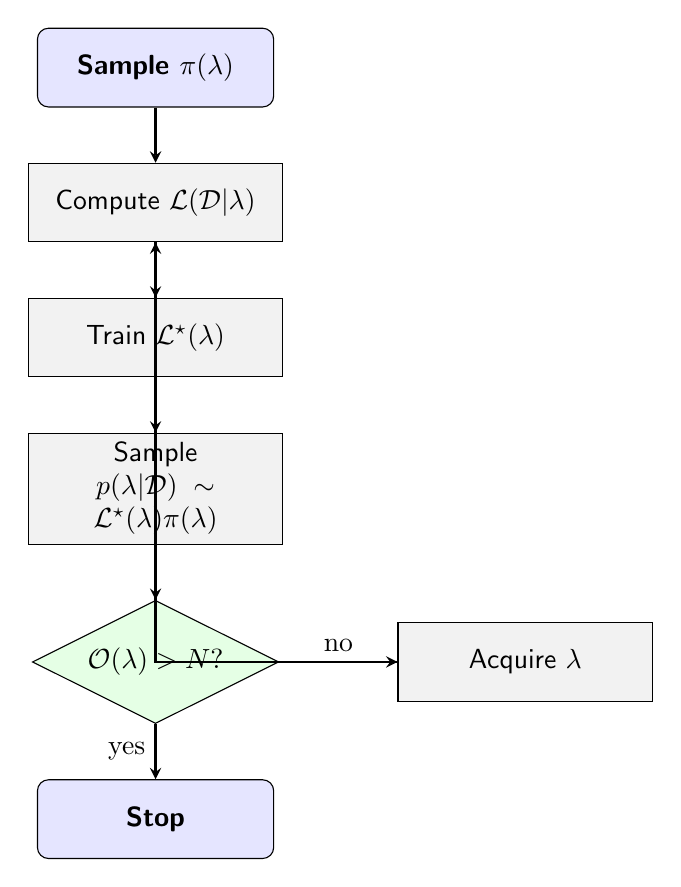
\begin{tikzpicture}[node distance=0.7cm and 1.5cm]
        \node (start) [startstop] {Sample $\pi(\lambda)$};
        \node (compute) [process, below=of start] {Compute $\Lmain$};
        \node (train) [process, below=of compute] {Train $\Lsurr$};
        \node (sample) [process, below=of train] {Sample\\$p(\lambda|\mathcal{D})\sim\Lsurr\pi(\lambda)$};
        \node (check) [decision, below=of sample] {$\mathcal{O}(\lambda) > N?$};
        \node (stop) [startstop, below=of check] {Stop};
        \node (acquire) [process, right=of check] {Acquire $\lambda$};

        \draw [arrow] (start) -- (compute);
        \draw [arrow] (compute) -- (train);
        \draw [arrow] (train) -- (sample);
        \draw [arrow] (sample) -- (check);
        \draw [arrow] (check) -- node[above] {no} (acquire);
        \draw [arrow] (check) -- node[left] {yes} (stop);
        \draw [arrow] (acquire) -| (compute);
    \end{tikzpicture}
    \caption{Flowchart of the process}
    \label{fig:flowchart}
\end{figure}

\subsection{Acquisition Functions}

An acquisition function is a function that maps the posterior predictive mean and variance to a scalar value. The scalar value is used to select the next point to observe from the model.

In general, we will write the acquisition function as $\alpha(\mu,\sigma)$, where $\mu$ is the posterior predictive mean and $\sigma$ is the posterior predictive variance.

Each criterion performs a trade-off between exploration i.e. investigating regions where the variance is large and exploitation i.e. investigating regions where the prediction is minimized. 

\paragraph{Uncertainty-based exploration (UE)}

This acquisition function aims at reducing the uncertainty of the GP model. It is defined as

$$
\alpha_{\rm{UE}}^i(\sigma^i)= \sigma^i
$$

and helps to explore the function space in regions of high uncertainty.

One of the most popular BO algorithms is the Efficient Global Optimization (EGO). 
It uses GP as surrogate model and the Expected Improvement as the infill sampling criterion. 


\paragraph{Expected Improvement}

This also focuses on the maximisation/minimisation of the GP's posterior predictive mean.
It looks for the best value of $\mu$ so far and then looks for the next point that has a higher probability of being better than the best value so far.

$$
\alpha_{\rm{EI}}^i(\mu^i, \sigma^i)= \sigma^i\ (u^i \mathcal{N}_{\rm CDF}(u^i) \mathcal{N}_{\rm PDF}(u^i)\ ,
$$

where $u^i = {(\mu^i - \mu{\rm{best})}}/{\sigma^i}$ and $\mu_{\rm{best}}$ is the best value of $\mu$ so far.

where $\mathcal{N}_{\rm PDF}$ denotes the Probability Density function (PDF) of the univariate Gaussian probability distribution.

While we would like to choose $x$ so that this improvement is large, $f(x)$ is unknown until after the evaluation.  What we can do, however, 
is to take the expected value of this improvement and choose $x$ to maximize it.

The Expected Improvement (EI)takes into account the improvement induced by a candidate that is defined as: $I(\textbf{x})=\text{max}\{0,y_{\text{min}}-f(\textbf{x})\}$. 












\subsection{Diagnostics}

We run an MCMC sampler using
\begin{equation}
    \mathcal{L}^{\star}(\lambda) = \mu_{\mathcal{GP}}(\lambda)
\end{equation}
\begin{equation}
    \mathcal{L}^{\star}_{V}(\lambda) = \mathcal{N}(\mu_{\mathcal{GP}}(\lambda), \sigma_{\mathcal{GP}}(\lambda))
\end{equation}


The KL divergence using the two \Lsurr should converge once the model is trained. 
Additionally, the KL divergence using a reference posterior trainined with a lot of points should converge.
This will indicate that the surrogate likelihood distribution has been adequately modelled in regions of parameter space. 


%--------------------------------------------------------
\section{Inference with surrogate model}
\label{sec:results}
\subsection{Simulation study}

To validate our method, we conduct the the study described in Section 2.5 of \citep{Riley:2023:ApJ}.

We simulate the evolution of 32 million binary systems using \COMPAS (settings specified in Appendix~\ref{sec:appendix_COMPAS_fiducial}), resulting in a population of approximately 68 thousand DCOs that merge within the age of the Universe, $\sim13.8\unit{Gyr}$. 
We sample 100 $\lambda$ from a $\pi(\lambda)$, and generate $\vec{\mathcal{D}}$, unique mock \COMPAS populations for each $\lambda$.
We build surrogate likelihoods for each dataset, and use them to approximate $p(\lambda|\mathcal{D})$.
Figure~\ref{fig:simulation_posterior} displays the $p(\lambda|\mathcal{D})$ for one mock population.
The gray ``reference'' posterior is obtained using a surrogate likelihood $\mathcal{L}^{\star}$ tranined with 950 points.
The blue posterior is obtained using a surrogate likelihood $\mathcal{L}^{\star}_V$ trained with 50 points, while the purple posterior's surrogate is built with 325 points. 
The blue posterior has a $D_{KL}>10$ when compared with the gray reference posterior. 
The purple  posterior has a $D_{KL}<1$ when compared with the gray reference posterior, indicating that the two posteriors are similar. 
The orange line marks the true $\lambda$ used to generate the dataset. 
\begin{figure}[ht!]
    \script{plot_simulation_posterior.py}
    \begin{centering}
        \includegraphics[width=\linewidth]{figures/simulation_posterior.pdf}
        \caption{
            Simulation posteriors
        }
        \label{fig:simulation_posterior}
    \end{centering}
\end{figure}


The PP-plot in Figure~\ref{fig:pp_plot} shows that the true value lies withing the correct region of the credible intervals, indicating that the results are not biased.
\begin{figure}[ht!]
    \script{plot_pp_plot.py}
    \begin{centering}
        \includegraphics[width=\linewidth]{figures/pp_plot.pdf}
        \caption{
            PP-plots from simulation study.
        }
        \label{fig:pp_plot}
    \end{centering}
\end{figure}


Finally, Figure~\ref{fig:kl_distances} shows the JS diveregence 

\begin{figure}[ht!]
    \script{plot_kl_distances.py}
    \begin{centering}
        \includegraphics[width=\linewidth]{figures/kl_distances.pdf}
        \caption{
            KL-Distances of the posteriors obtained with XX, compared against to those from YY.
        }
        \label{fig:kl_distances}
    \end{centering}
\end{figure}












%--------------------------------------------------------
\subsection{LVK analysis}
\paragraph{Data}

The catalogue of LIGO, Virgo, and KAGRA (LVK) gravitational wave observations (\citet{GWTC-2_1_zenodo}, \citet{GWTC-3_zenodo}) provides us with a number of merger detections from a population of \acp{DCO}. 
 For each LVK event we know, among other things, the chirp mass of the merging binary and the merger redshift, up to a measurement uncertainty.
We get the data from the \ogc.
Plots of the event $\Mc,z$ median estimates and $X-\sigma$ uncertainty can be found in Figure~\ref{fig:ogc4_events}. 
Filtering the events based on the OGC definition of $p(bbh)\geq0.95$ and ensuring that the median value of the $p(\Mc,z|d_i)$ lies within $\Mc\in[4,45]$, $z\in[0,1]$, we get XX events. 
Less confident events could be included \citep[e.g.][]{Farr_2015}, they will typically contribute little information due to greater measurement uncertainties.
These events that we use in our analysis are colored green in Fig~\ref{fig:ogc4_events}.

\begin{figure}[ht!]
    \script{plot_ogc4_events.py}
    \begin{centering}
        \includegraphics[width=0.8\columnwidth]{figures/ogc4_events.pdf}
        \caption{
            The events and uncertainty as predicted by Ogc4
        }
        \label{fig:ogc4_events}
    \end{centering}
\end{figure}

The priors for the events are in $\pi(\Mc,V_c)$, however, we need $\pi(\Mc,z)$. To transform the priors, we use the following equation
\begin{equation}
    \pi(\Mc,z) = \pi(\Mc, V_c(z)) \frac{d V_c(z)}{dz}\, .
\end{equation}
We use the definition of $d V_c(z)/dz$ from \citep{Hogg:1999:arXiv}, given by 
\begin{equation}
dV_{\rm C}= D_{\rm H}\,\frac{(1+z)^2\,D_{\rm A}^2}{E(z)}\,d\Omega\,dz
\end{equation}


Using Equation~\ref{eq:weights}, we obtain the weights for each posterior. 
A plot of each event's weights summed together is shown in Figure~\ref{fig:ogc4_weights}.




\begin{figure}[ht!]
    \script{plot_ogc4_weights.py}
    \begin{centering}
        \includegraphics[width=\linewidth]{figures/ogc4_weights.pdf}
        \caption{
            Weights generated using the OGC4 posteriors
        }
        \label{fig:ogc4_weights}
    \end{centering}
\end{figure}


\paragraph{Posteriors}
pass


%--------------------------------------------------------
\section{Discussion}
\label{sec:discussion}

Future work
\begin{itemize}
    \item Do hyper-parameter optimisation for the GP (kernal choices, kernel settings) 
    \item Do hyper-parameter optimisation for the acquisition function 
    \item Explore range of acquisition functions
\end{itemize}


%%% DATA AVAILABILITY %%%
\section*{Data availability}
The data underlying this article is available in the Zenodo deposit for this work. LINK TO ZENODO.

\section*{Acknowledgements}
We gratefully acknowledge the Swinburne Supercomputing OzSTAR Facility for computational resources. All analyses (including test and failed analyses) performed for this study used $XX$K core hours on OzSTAR. This would have amounted to a carbon footprint of ${\sim XX{\text{t CO}_2}}$~\citep{greenhouse, energy_to_co2_converter}. Thankfully, as OzSTAR is powered by wind energy from Iberdrola Australia; the electricity for computations produces negligible carbon waste.
4-OGC.
IM is a recipient of the Australian Research Council Future Fellowship FT190100574.
AV is XX.
Discussions with Renate, Matt, Kate.



\vspace{5mm}
\facilities{LIGO-VIRGO-KAGRA}
%
\software{
\python~\citep{pythonForScientificComputing,pythonForScientists},
\astropy~\citep{astropy},
\COMPAS~\citep{COMPAS_SOFTWARE_2022},
\pycbc~\citep{},
\emcee~\citep{},
\trieste~\citep{},
\tensorflow~\citep{},
\numpy~\citep{numpy},
\scipy~\citep{SciPy},
\pandas~\citep{pandas},
\matplotlib~\citep{matplotlib},
\corner~\citep{corner},
\sphinx~\citep{sphinx_doc},
\jupyterbook~\citep{jupyter,jupyter_book}.
}







\bibliography{bib}

\appendix



\section{COMPAS configuration fiducial values}\label{sec:appendix_COMPAS_fiducial}

\begin{table*}[ht!]
\centering
\caption{Initial values and default settings for the \COMPAS fiducial model.}
%
\label{tab:app_COMPAS_fiducial}
% ?\textwidth}{l @{\extracolsep{\fill}}
\resizebox{\textwidth}{!}{%
% \begin{adjustbox}{max width=1\textwidth}
% \centering
\begin{tabular}{lll}
\hline  \hline
Description and name                                 														& Value/range                       & Note / setting   \\ \hline  \hline
\multicolumn{3}{c}{Initial conditions}                                                                      \\ \hline
Initial primary mass \monei                               															& $[5, 150]$\Msun    & \citet{Kroupa_2001} IMF  $\propto  {\monei}^{-\alpha}$  with $\alpha_{\rm{IMF}} = 2.3$ for stars above $5$\Msun	  \\
%
Initial mass ratio $\qi = \mtwoi / \monei $           												& $[0, 1]$                          &       We assume a flat mass ratio distribution  $p(\qi) \propto  1$ with \mtwoi $\geq 0.1\Msun$   \\
%
Initial semi-major axis \ai                                            											& $[0.01, 1000]$\AU & Distributed flat-in-log $p(\ai) \propto 1 / {\ai}$ \\
%
Initial metallicity \Zi                                           											& $[0.0001, 0.03]$                 & Distributed uniform-in-log   \\
%
Initial orbital eccentricity \ei                                 							 				& 0                                & All binaries are assumed to be circular at birth  \\
%
% initial rotation of stars                            															& 0                                 &                  \\  \hline
\hline
%initial mass function (IMF) slope 	$\alpha_{\rm{IMF}}$									&  $ 2.3$		& 	 for stars above $5$\Msun from \citet{2001MNRAS.322..231K} IMF\\  \hline
\multicolumn{3}{c}{Fiducial parameter settings:}                                                            \\ \hline
%
Stellar winds  for hydrogen rich stars                                   																&      \citet{Belczynski_2010a}    &   Based on {\citet{Vink_2000, Vink_2001}}, including  LBV wind mass loss with $f_{\rm{LBV}} = 1.5$   \\
%
Stellar winds for hydrogen-poor helium stars &  \citet{Belczynski_2010a} & Based on   {\citet{Hamann_1998}} and  {\citealt{Vink_2005}}  \\

%%%%%%%%%%%%%%%%%%%%%%%%%%%%%%%%%%%%%%%%%%%%%%%%
%%%%%%%%%%%%%% MASS TRANSFER THINGS %%%%%%%%%%%%%%%%%%%%%%%
%
Max transfer stability criteria & $\zeta$-prescription & Based on \citet[][]{Vigna-Gomez_2018} and references therein     \\
%
Mass transfer accretion rate & thermal timescale & Limited by thermal timescale for stars  \citet[][]{Hurley_2002, Vinciguerra_2020} \\
 & Eddington-limited  & Accretion rate is Eddington-limit for compact objects  \\
%
Non-conservative mass loss & isotropic re-emission &  {\citet[][]{Massevitch_1975, Bhattacharya_1991, Soberman_1997}} \\
& &  {\citet{Tauris_2006}} \\
%
Case BB mass transfer stability                                														& always stable         &       Based on  \citet{Tauris_2015, Tauris_2017, Vigna-Gomez_2018}         \\
%
%%%%%%%%%%%%%%%%%%%%%%%%%%%%%%%%%%%%%%%%%%%%%%%%
%%%%%%%%%%%%%% CE THINGS %%%%%%%%%%%%%%%%%%%%%%%
%
CE prescription & $\alpha-\lambda$ & Based on  \citet{Webbink_1984, deKool_1990}  \\
%
CE efficiency $\alpha$-parameter                     												& 1.0                               &              \\
%
CE $\lambda$-parameter                               													& $\lambda_{\rm{Nanjing}}$                             &        Based on \citet{Xu_2010a, Xu_2010b} and  \citet{Dominik_2012}       \\
%
Hertzsprung gap (HG) donor in {CE}                       														& pessimistic                       &  Defined in \citet{Dominik_2012}:  HG donors don't survive a {CE}  phase        \\
%
%%%%%%%%%%%%%%%%%%%%%%%%%%%%%%%%%%%%%%%%
%%%%%%%%%.    SN THINGS   %%%%%%%%%%%%%%
%%%%%%%%%%%%%%%%%%%%%%%%%%%%%%%%%%%%%%%%
%
{SN} natal kick magnitude \vk                          									& $[0, \infty)$\kms & Drawn from Maxwellian distribution with standard deviation $\sigma_{\rm{rms}}^{\rm{1D}}$          \\
%
 {SN} natal kick polar angle $\thetak$          											& $[0, \pi]$                        & $p(\thetak) = \sin(\thetak)/2$ \\
%
 {SN} natal kick azimuthal angle $\phi_k$                           					  	& $[0, 2\pi]$                        & Uniform $p(\phi) = 1/ (2 \pi)$   \\
%
 {SN} mean anomaly of the orbit                    											&     $[0, 2\pi]$                             & Uniformly distributed  \\
 %
Core-collapse  {SN} remnant mass prescription          									     &  delayed                     &  From \citet{Fryer_2012}, which  has no lower {BH} mass gap  \\%
%
USSN  remnant mass prescription          									     &  delayed                     &  From \citet{Fryer_2012}   \\%
%
ECSN  remnant mass presciption                        												&                                 $m_{\rm{f}} = 1.26\Msun$ &      Based on Equation~8 in \citet{Timmes_1996}          \\
%
Core-collapse  {SN}  velocity dispersion $\sigma_{\rm{rms}}^{\rm{1D}}$ 			& 265\kms           & 1D rms value based on              \citet{Hobbs_2005}                          \\
%
 USSN  and ECSN  velocity dispersion $\sigma_{\rm{rms}}^{\rm{1D}}$ 							 	& 30\kms             &            1D rms value based on e.g.,    \citet{Pfahl_2002, Podsiadlowski_2004}    \\
%
PISN / PPISN remnant mass prescription               											& \citet{Marchant_2019}                    &       As implemented in \citet{Stevenson_2019}      \\
Maximum NS mass                                      & $\rm{max}_{\rm{NS}} = 2.5$\Msun & Following \citet{Fryer_2012}            \\
Tides and rotation & & We do not include tides and/or rotation in this study\\
Binary fraction                                      & $f_{\rm{bin}} = 0.7$ &  \\
Solar metallicity \Zsun                             & $\rm{Z}_{\odot}\xspace = 0.0142$ & based on {\citet{Asplund_2009}} \\
%
%
\hline
\multicolumn{3}{c}{Simulation settings}                                                                     \\ \hline
Binary population synthesis code                                      & COMPAS &       \citet{Stevenson_2017, Barrett_2018, Vigna-Gomez_2018, Neijssel_2019} \\
& & \citet{Broekgaarden_2019, COMPAS_2022}.        \\
\hline \hline
\end{tabular}%
% \end{adjustbox}
}
\end{table*}



\section{Sampler settings}\label{sec:appendix_sampler_settubgs}
Here we describe the sampler settings we use. 
We also plot some trace plots.


\section{Posteriors}

% \begin{figure}[htbp]
%     \centering
%     \begin{subfigure}{0.45\textwidth}
%         \centering
%         \includegraphics[width=\textwidth]{figures/5M_50_940pts.pdf}
%         \caption{First image}
%         \label{fig:image1}
%     \end{subfigure}
%     \hfill
%     \begin{subfigure}{0.45\textwidth}
%         \centering
%         \includegraphics[width=\textwidth]{figures/32M_50_780pts.pdf}
%         \caption{Second image}
%         \label{fig:image2}
%     \end{subfigure}
%     \caption{Posteriors for MSSFR parameters using LVK data}
%     \label{fig:two_images}
% \end{figure}


\begin{figure}[htb]
    \centering
    \begin{minipage}{0.45\columnwidth}
        \includegraphics[width=\linewidth]{figures/5M_50_940pts.pdf}
        \caption{Caption for subfigure (a)}
    \end{minipage}\hfill
    \begin{minipage}{0.45\columnwidth}
        \includegraphics[width=\linewidth]{figures/32M_50_780pts.pdf}
        \caption{Caption for subfigure (b)}
    \end{minipage}
    \caption{Main caption for the entire figure}
    \label{fig:main}
\end{figure}



\end{document}
